
\section{Discrete Laplacians}\label{sec:Chapter3: other discrete laplacians}
\subsection{The Equivariance error for graph convolutions}
Take a sampling scheme $V=\{v_i\in\mathbb S^2, i=0, ..., n\}$ of the sphere, a weighted undirected graph $G(V, E, \mathbf W)$, a signal $f: \mathbb S^2\to\mathbb R$ and its sampled representation $\mathbf f:\ f_i=f(v_i)$. Suppose that there exists a sampling operator $T_V: L^2(\mathbb S^2) \supset F\to \mathbb R^n,\  T_V(f) = \mathbf f$ defined on a suitable subspace $F$ of $L^2(\mathbb S^2)$ such that it is invertible, i.e., we can unambiguously reconstruct the function $f\in F$ from its sampled values $\mathbf f$. The existence of such subspace depends on the sampling scheme $V$, and its characterization is a common problem in signal processing \cite{Driscoll:1994:CFT:184069.184073}. Recall the definition (\ref{eq:rotation operator}) of the rotation operator $\Lambda(g), g\in SO(3)$. 

We now want to understand how to set the edges and the weights of $G$ such that
\begin{equation}\label{eq:equivariance}
	T \Lambda(g) T^{-1} \Omega_k T f = \Omega_k T \Lambda(g) f
\end{equation}
i.e., the graph convolution $\Omega_k$ and any rotation $\Lambda(g)$ commute.
 
Verifying equation (\ref{eq:equivariance}) is really hard in practice, due to the fact that for almost all samplings schemes $V$ it is not known if there exists a space $F$ in which $T$ is invertible. A special case is the \textit{equiangular sampling} scheme described in section \ref{sec:Chapter3: Heat Kernel Graph Laplacian on the Equiangular Sampling} where the sampling theorem \ref{theo:equiangular sampling theorem} holds \cite{Driscoll:1994:CFT:184069.184073}. With all the other sampling schemes, there are no sampling theorems available but there are implementations of approximated, discrete SHT to reconstruct a sampled signal $\mathbf f$, thus providing a way to approximate $T^{-1}$. Thanks to this we are able, for a given sampling, a given function $f$ and a given rotation $g$, to compute the \textit{normalized equivariance error} 
\begin{equation}\label{eq:equivariance error}
	E_{G}(f, g) = \left(\frac{ \norm {T \Lambda(g) T^{-1} \Omega_k Tf - \Omega_k T \Lambda(g) f}_{L^2(\mathbb R^2)}}{\norm {Tf}_{L^2(\mathbb R^2)}}\right)^2
\end{equation}
where $T^{-1}$ is substituted with a discrete SHT in case $T$ is not invertible.
A measure of how equivariant a graph is with respect to rotations will then be given by the \textit{mean equivariance error}
\begin{equation}\label{eq:mean equivariance error}
\overline E_G = \mathbb E_{f, g}\ 	E_G(f, g) 
\end{equation}
In practice the expected value is obtained by averaging over a finite number of random functions and random rotations. The mean equivariance error $\overline E_G$ gives us an indication of how close the graph $G$ is from being equivariant to rotations.

Now we state an intuitive concept that explains how to construct rotation invariant graphs, i.e. graphs such that $\overline{E_G}$ is small.
\begin{snugshade*}
The mean equivariance error $\overline{E_G}$ will be small if the scalar product $\mathbf f^T \mathbf v_{i(\ell, m)}$ well approximates $\hat {f}(\ell,m)$ i.e., the $L^2$ scalar product of the continuous signal \\
$\hat {f}(\ell,m)= \int_{\eta \in \mathbb S^2}f(\eta)Y_\ell^m(\eta)d\mu(\eta)$.

\textit{If $V$ is an equal area sampling scheme}, i.e. the area around each pixel $v_i$ is the same, $\overline{E_G}$ will be small if the graph Laplacian $\mathbf L$ is such that its eigenvectors $\mathbf v_i$ well approximate the eigenfunctions of the Laplace-Beltrami operator $\Delta_{\mathbb S^2}$ evaluated in the points of the sampling scheme, i.e., 
$$
\mathbf v_{i(\ell, m)} \approxeq Y_\ell^m(x_i)
$$
\end{snugshade*}

In this way we framed the problem of constructing a rotation invariant graph with the more general problem of coming up with a matrix $\mathbf L$ with some specific spectral properties. Graphs are only one of many ways of coming up with such matrix $\mathbf L$, and many other methods have been already studied in the literature. In this section we present a brief overview of some of these methods providing the general context in which graph filtering can be framed.

Let $f$ be a sufficiently smooth function on a compact, closed infinitely differentiable manifold $\mathcal M$. The Laplacian eigenvalue problem on $\mathcal M$ is defined as 
\begin{equation}\label{eq:continous eigenvalue problem}
	\triangle_{\mathcal M}\psi = -\lambda \psi
\end{equation}
Being the Laplace-Beltrami operator self-adjoint and semi-positive definite, there exists a basis $\mathcal B=\{\psi_i\}_i$of the space $L^2(\mathcal M)$ such that $\triangle_\mathcal M \psi_i = -\lambda_i\psi_i,\ \lambda_0\leq\lambda_1\leq...,\lambda_i\leq\lambda_{i+1}...\leq+\infty$. See \cite{rosenberg_1997} for an introduction to the Laplace-Beltrami operator on manifolds.

There's been a lot of work in trying to calculate solutions to equation (\ref{eq:continous eigenvalue problem}), leading to different ways to approximate the Laplace-Beltrami operator through what we call a \textit{discrete Laplacian}. By discrete Laplacian we mean an operator $L$ that, once evaluated on a signal $f$ and on a vertex $x_i$ can be written as a matrix $\mathbf L$ in the following way:

\begin{equation}\label{eq:discrete laplacian}
	L f\left(\mathbf{x}_{i}\right)=\frac{1}{d_{i}} \sum_{j} w_{i j}\left(f\left(\mathbf{x}_{i}\right)-f\left(\mathbf{x}_{j}\right)\right)
\end{equation}

Note that with unit \textit{masses} $d_i=1$ we recover the same definition of Graph Laplacian. Before continuing the discussion we need to introduce some basic concepts of Differential Geometry, especially the definition of mean curvature of a manifold and its link with the Laplace-Beltrami operator.

\subsection{Notions of Differential Geometry}

 For this short introduction to basic concepts of Differential Geometry, set the manifold $\mathcal M$ to be a differentiable, two dimensional surface embedded in $\mathbb R^3$. 
 \begin{figure}[h]
 	\centering
 	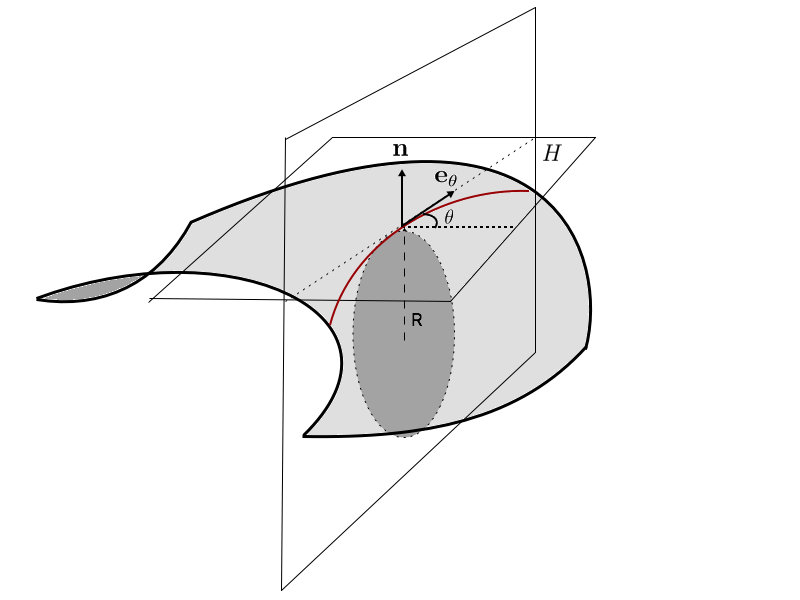
\includegraphics[width=0.7\textwidth]{figs/Chapter3/curvature.png}
 	\caption{\label{fig:curvature}Curvature normal of a manifold}
 \end{figure} 
The \textit{curvature} of a curve on a plane is defined as the inverse of the radius $R$ of the tangent circle. For each point on the manifold $\mathcal M$, define its tangent plane $H$, orthogonal to the normal vector $\mathbf n$. For every unit vector $\mathbf e_\theta$ lying on the tangent plane $H$, where $\theta$ is an angle that measures the direction on the tangent plane of $\mathbf e_\theta$, the \textit{normal curvature} $\kappa(\theta)$ is defined as the curvature of the curve that is the intersection of the manifold $\mathcal M$ and the plane containing both $\mathbf n$ and $\mathbf e_\theta$. The \textit{mean curvature} $\overline \kappa $ is defined as the average on $\theta$ of the normal curvatures:
 
 \begin{equation}\label{eq:mean curvature}
 	\overline \kappa=\frac{1}{2 \pi} \int_{0}^{2 \pi} \kappa(\theta) d \theta
 \end{equation}

It can be proved that the Laplace-Beltrami operator applied on the identity function $\mathbf x \rightarrow \mathbf x, \ \forall \mathbf x\in \mathcal M$ is directly linked to the \textit{mean curvature normal} $\overline{\kappa}\mathbf n$ by the following formula:
\begin{equation}\label{eq:laplacian and curvature}
	\triangle_\mathcal M \mathbf x  = -2\overline{\kappa}\mathbf n
\end{equation}
This equation provides us a way to approximate the Laplace-Beltrami operator through the approximation of the mean curvature normal. This fact is exploited by methods presented in the next section.

\subsection{Discrete Laplacians from Differential Geometry}
\begin{figure}[h]
	\begin{center}
		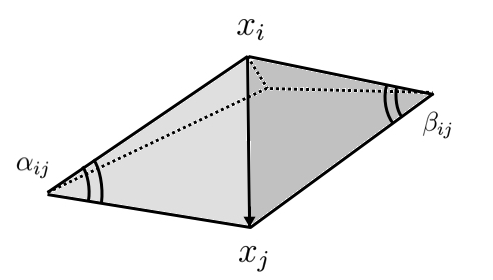
\includegraphics[width=0.45\textwidth]{figs/Chapter3/MyDesbrun.png}
		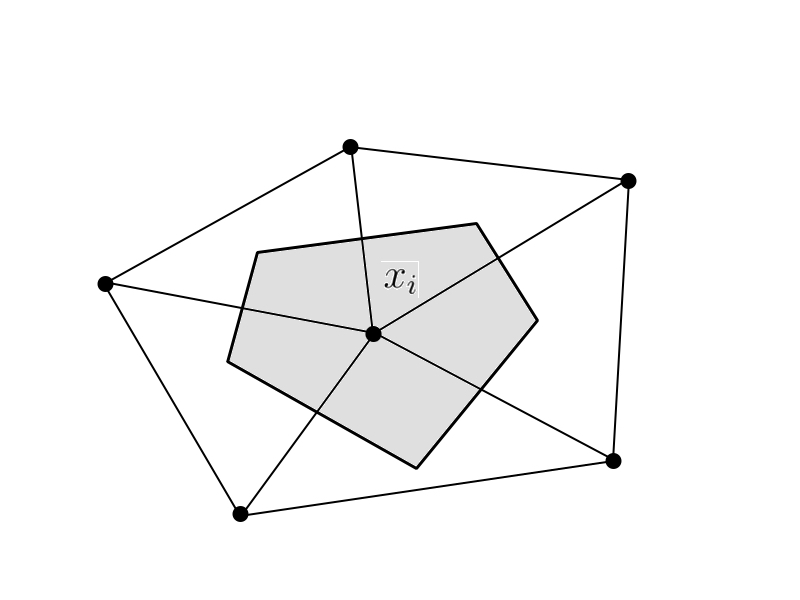
\includegraphics[width=0.45\textwidth]{figs/Chapter3/Voronoi}
	\end{center}
	\caption{\label{fig:Desbrun}One term of curvature normal formula and one Voronoi cell constructed around the node $x_i$}
\end{figure} 
Desbrun et al. \cite{Desbrun1999} construct a triangulation $\mathcal T_h$ with the vertices in the sampling $x_0, x_1, ..., x_{n-1}$ approximating the manifold $\mathcal M$, and then use the following discrete expression for the \textit{discrete normal curvature} $\overline{\kappa_h} \mathbf{n}$ of the manifold $\mathcal M$:
\begin{equation}\label{eq:curvature normal}
	-\overline{\kappa_h} =\frac{1}{4 A_i} \sum_{j \in N_{1}(i)}\left(\cot \alpha_{ij}+\cot \beta_{ij}\right)\left(x_{j}-x_{i}\right)
\end{equation}
where $A_i$ is the area of all the triangles of the mesh sharing the node $x_i$; $N_1(i)$ is the first ring of neighbors of the i-th node; $\alpha_{i j},\ \beta_{i j}$ are the angles of the triangles of the mesh that lie on the opposite side to the edge $(i,j)$ with respect to the node $x_i$ (Figure \ref{fig:Desbrun}). Observe that for a flat surface the discrete curvature is equal to zero $\overline{\kappa_h}=0$. This is a geometric approach that relies on the intrinsic properties of the triangulation $\mathcal T_h$ and is based on the geometric meaning of the curvature normal $\overline{\kappa}$. Using equations (\ref{eq:curvature normal}) and (ref{eq:laplacian and curvature}) it can be shown \cite{REUTER2009381} that this approach leads to a \textit{discrete Laplacian} with masses $d_i=A_i$ where $A_i$ is the area of all the triangles of the mesh with a node in $x_i$, and weights
$$
w_{i j}=\frac{\cot \left(\alpha_{i j}\right)+\cot \left(\beta_{i j}\right)}{2}
$$

Meyer et al. \cite{Meyer02discretedifferential-geometry} modify the masses of Desbrun et al. and set the masses $d_i$ to be equal to $a_{V}(i)$, where \(a_{V}(i)\) is the area of the polygon obtained by joining the circumcenters of the triangles surrounding node $i$ (i.e. the Voronoi cell, figure \ref{fig:Desbrun}).

\subsection{Linear Finite Element Method Laplacian}
The eigenvalue problem (\ref{eq:continous eigenvalue problem}) can be rewritten in the equivalent weak form
\begin{equation}\label{eq:weak}
	\langle \nabla f, \nabla v\rangle_{L^2(\mathbb S^2)} = \lambda \langle  f, v\rangle_{L^2(\mathbb S^2)} \quad \forall v \in L^2(\mathbb S^2)
\end{equation}
The Finite Element Method (FEM) is a numerical algorithm that allows to calculate a discrete approximation of the solution $f$ through a functional discretization of the weak eigenvalue problem (\ref{eq:weak}). We will discuss this method deeper in section \ref{sec:Chapter3: Using the Finite Element Method to approximate the Laplace-Beltrami operator on a manifold}. By projecting equation (\ref{eq:weak}) on a finite dimensional functional subspace of $L^2(\mathbb S^2)$ spanned by $n$ basis functions $\phi_i$, by writing $n$ times the equation (\ref{eq:weak eigenvalue problem}), setting each time the \textit{test} function $v$ equal to the $i$th basis function $\phi_i$ we obtain the generalized algebraic eigenvalue problem
$$
\begin{aligned}
&\text{Find }(f,\lambda)\text{ such that }A\mathbf f = \lambda B \mathbf f\\
&\begin{cases}
(A)_{ij} &= \int_{\mathbb S^2}\nabla \phi_i(\mathbf{x})\cdot \nabla \phi_j(\mathbf{x})d\mathbf{x}\\
(B)_{ij} &= \int_{\mathbb S^2} \phi_i(\mathbf{x}) \phi_j(\mathbf{x})d\mathbf{x}\\
(\mathbf f)_i &= f_i:\quad f(\mathbf x) = f_0\phi_0(\mathbf x)+ ... + f_{n-1}\phi_{n-1}(\mathbf x) 
\end{cases}
\end{aligned}
$$
that can be solved through usual algebraic solvers.

\subsection{Graph Laplacian for manifolds}\label{sec:Chapter1:theoretical foundations}
In their work, Convergence of Laplacian Eigenmaps \cite{NIPS2006_2989}, Belkin et al. prove convergence of eigenvectors of the \textit{Heat Kernel Graph Laplacian} $\mathbf L_n^t$ (HKGL) of a data point cloud to the eigenfunctions of the Laplace Beltrami operator $\Delta_\mathcal M$ on the manifold $\mathcal M$, when the data is sampled from a uniform distribution on $\mathcal M$.
For this result to hold, they suppose the manifold $\mathcal M$ to be compact, infinitely differentiable and without boundary. We just point out that being $\mathcal M$ compact, $\Delta_\mathcal M$ has a discrete spectrum. The graph they use to approximate the manifold is constructed as follows: given a sampling $ \mathcal P = \{x_i\in\mathcal M\}_{i=0}^{n-1}$ on a $k$-dimensional manifold $\mathcal M\subset \mathbb R^N$ they construct the full graph defined by the weights 
$$
w_{ij}=\exp\left({-\frac{||x_i-x_j||^2}{4t}}\right)
$$
where $\norm\cdot$ is the Euclidean norm in the ambient space $\mathbb R^N$ and whose Laplacian matrix 
$$
\mathbf L_n^t = \mathbf D-W
$$ we call \textit{Heat Kernel Graph Laplacian}.

Observe that given a function $f: \mathcal P \rightarrow \mathbb R$ defined on the sampling $ \mathcal P$ and defined the vector $\mathbf f\in\mathbb R^n$ such that $\mathbf f_i = f(x_i)$, the Heat Kernel Graph Laplacian matrix acts on $\mathbf f$ in the following way:
\begin{equation}\label{eq:HKGL}
(\mathbf L_n^t \mathbf f)_i:=  \sum_{j=0}^{n-1} e^{-\frac{||x_i-x_j||^2}{4t}}\left(f(x_i)-f(x_j)\right)
\end{equation}
This graph construction is motivated by the fact that the HKGL is nothing else than the natural discretization of the continuous \textit{functional approximation to the Laplace-Beltrami operator} $L^t:  L^{2}(\mathcal{M}) \rightarrow L^{2}(\mathcal{M})$ that is proven to converge to $\Delta_\mathcal M$.
\vspace{0.5cm}
\begin{definition}{}(\cite[Belkin et al.]{Belkin:2005:TTF:2138147.2138189}Functional approximation to the Laplace-Beltrami operator)\\ \label{eq: my L^t} Let $\mu$ be the uniform probability measure on the manifold $\mathcal M$, where $\text{vol}(\mathcal M)$ is the volume of $\mathcal M$. We define the functional approximation to the Laplace-Beltrami operator to be the operator $L^t: L^{2}(\mathcal{M}) \rightarrow L^{2}(\mathcal{M})$ such that
	\label{def:Functional approximation to the Laplace-Beltrami operator}
	$$ L^tf(y) = \int_{\mathcal M}e^{-\frac{||y-x||^2}{4t}}\left(f(y)-f(x)\right)d\mu(x)$$
\end{definition}
We end this Chapter by stating the theorem of spectral convergence of the HKGL to the Laplace-Beltrami operator $\Delta_\mathcal M$, that makes it a really good candidate to construct rotation invariant graphs.
\vspace{0.5cm}
\begin{snugshade*}
	\begin{theorem}(Belkin et al., \cite{NIPS2006_2989})\label{theo:spectral convergence}
		Let \(\lambda_{n, i}^{t}\) be the $i$th eigenvalue of 
		$$
		\frac{(4\pi t)^{-(k+2)/2}}{n}\mathbf L^t_n
		$$
		and \(\mathbf v_{n, i}^{t}\) be the corresponding eigenvector. Let \(\lambda_{i}\) and \(v_{i}\) be the corresponding eigenvalue and eigenfunction of \(\Delta\) respectively. Then there exists a sequence \(t_{n} \rightarrow 0,\) such that
		\begin{equation}
		\begin{array}{c}{\lim _{n \rightarrow \infty} \lambda_{n, i}^{t_{n}}=\lambda_{i}} \\ 
		{\lim _{n \rightarrow \infty}\left\|\mathbf v_{n, i}^{t_{n}}-v_{i}(\mathbf x)\right\|_{2}=0}\end{array}
		\end{equation}
		where the limits are in probability.
	\end{theorem}
\end{snugshade*}



